\newthought{\textbf{Arya Saputra - 2020903430009 - TRKJ 3B}}

\newday{\textbf{1 -2 Desember 2022} - Instalasi dan Konfigurasi Hadoop}
\begin{enumerate}
\item Kendala dan Solusi \\
Pada pertemuan hari ini, kegiatan yang dilakukan adalah menginstall Apache Hadoop. Selama praktikum tidak mengalami kendala.

\item Kesimpulan
Berhasil melakukan instalasi hadoop berikut ini gambar hasil verifikasi instalasi hadoop version.
\end{enumerate}

\begin{figure}[!ht]
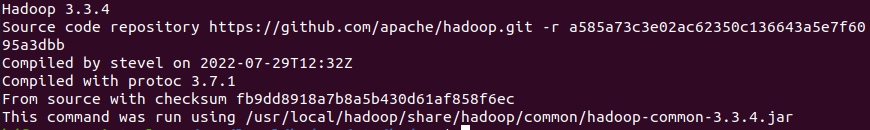
\includegraphics[width=\textwidth]{AryaSaputra/hadoop version}
\caption{Verifikasi Hasil Instalasi Hadoop}
\label{gam:Hadoop-version}
\end{figure}

\begin{figure}[!ht]
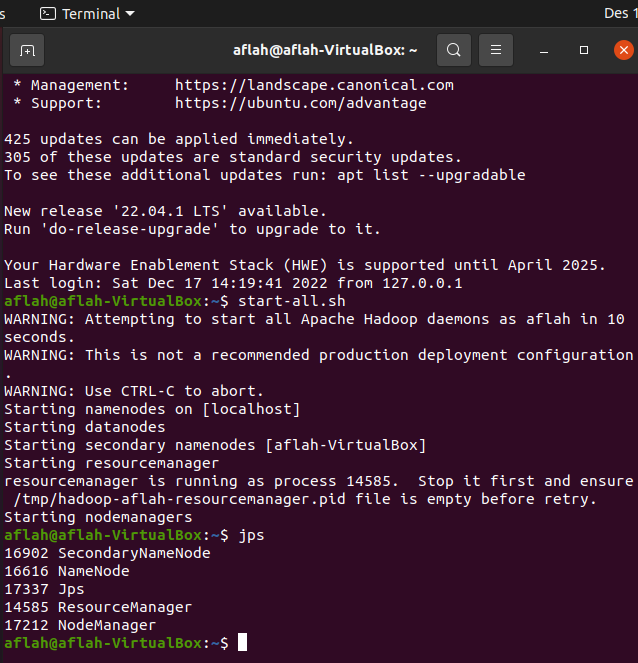
\includegraphics[width=\textwidth]{AryaSaputra/jps}
\caption{Verifikasi Hasil Instalasi Hadoop}
\label{gam:instalasi-hadoop}
\end{figure}

\begin{figure}[!ht]
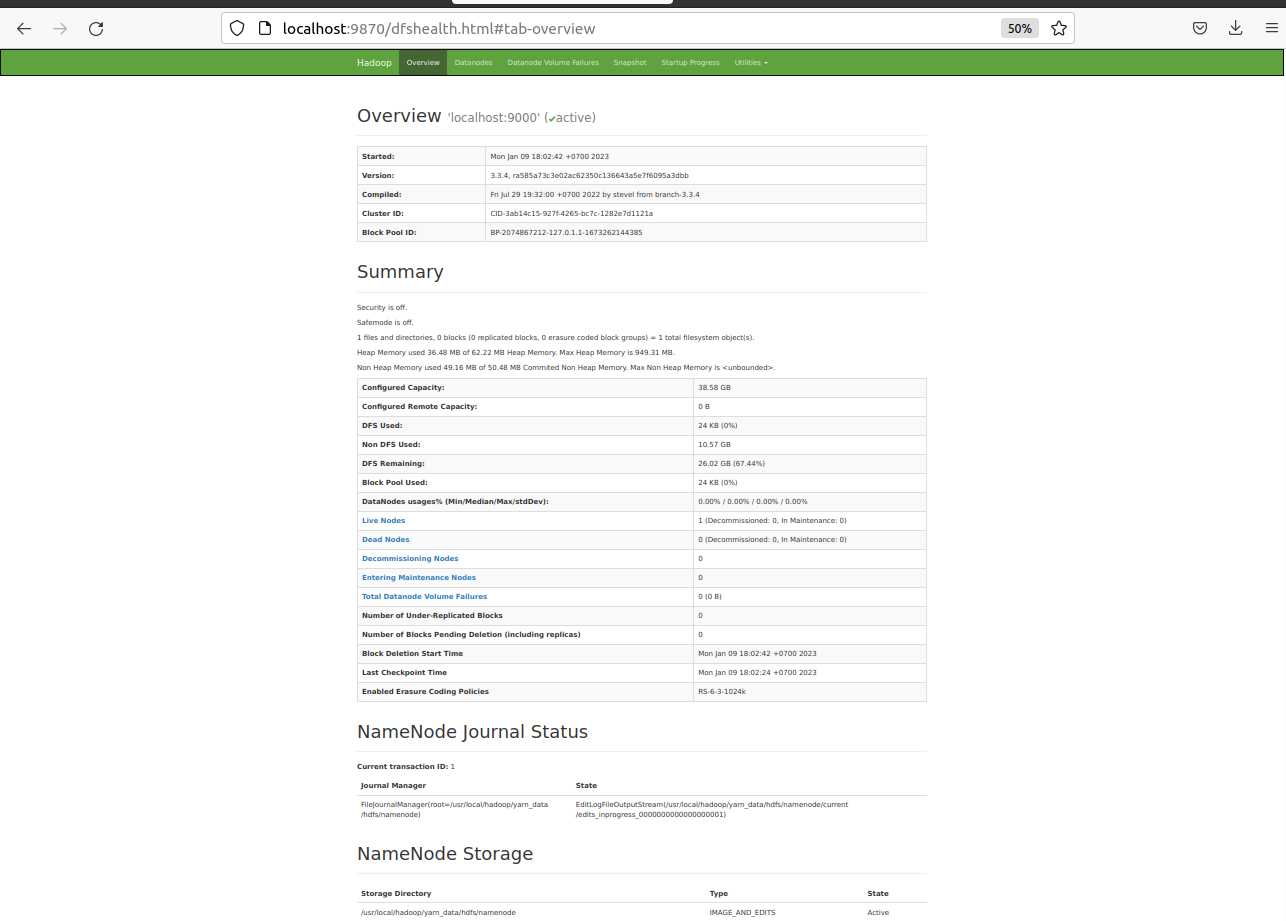
\includegraphics[width=\textwidth]{AryaSaputra/localhos1}
\caption{Verifikasi Hasil Instalasi Hadoop}
\label{gam:instalasi-hadoop}
\end{figure}

\begin{figure}[!ht]
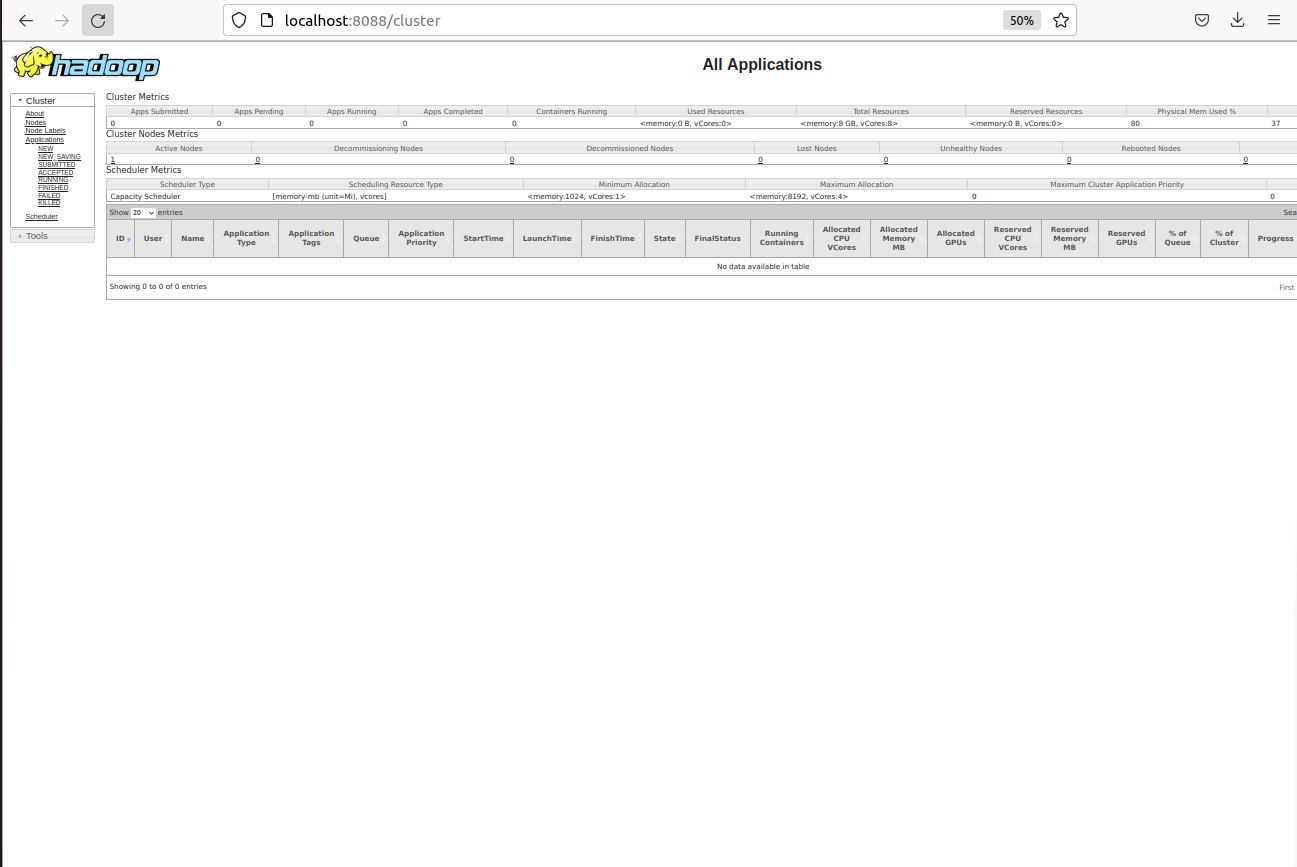
\includegraphics[width=\textwidth]{AryaSaputra/localhos2}
\caption{Verifikasi Hasil Instalasi Hadoop}
\label{gam:instalasi-hadoop}
\end{figure}

\newday{\textbf{15 Desember 2022} - WordCount Bawaan Java}
\begin{enumerate}
\item Kendala dan Solusi
\newline Tidak ada kendala apapun saat melakukan program WordCount bawaan Hadoop

\item Kesimpulan
\newline Praktikum berhasil dilakukan sesuai dengan perintah-perintah yang ada. WordCount sendiri merupakan program untuk menghitung jumlah kata yang ada pada data.

\begin{figure}[!ht]
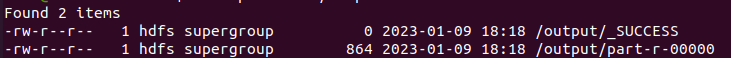
\includegraphics[width=\textwidth]{AryaSaputra/cek hasil wordcount bawaan}
\caption{Hasil dari langkah 6}
\label{gam:wordcount bawaan}
\end{figure}

\begin{figure}[!ht]
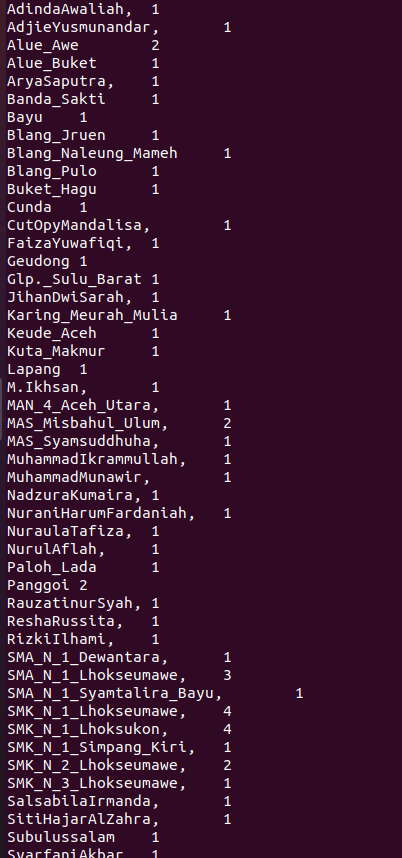
\includegraphics[width=.65\textwidth]{AryaSaputra/hasil wordcount bawaan}
\caption{Hasil dari langkah 7}
\label{gam:wordcount bawaan}
\end{figure}

\vspace*{-1cm}
\begin{figure}[!ht]
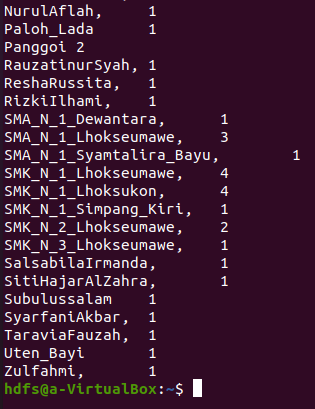
\includegraphics[width=.55\textwidth]{AryaSaputra/2}
\caption{Hasil dari langkah 7}
\label{gam:wordcount bawaan}
\end{figure}
\end{enumerate}

\clearpage
\newday{\textbf{16 Desember 2022} - WordCount dengan Java}
\begin{enumerate}
\item Kendala dan Solusi
\newline Kendala :
Saat melakukan praktikum program WordCount dengan Java tidak ada kendala saat melakukan pratikum.

\item Kesimpulan
\newline Praktikum berhasil dilakukan sesuai dengan perintah-perintah yang ada. Data pada WordCount dapat ditampilkan sesuai dengan yang telah dibuat.


\begin{figure}[!ht]
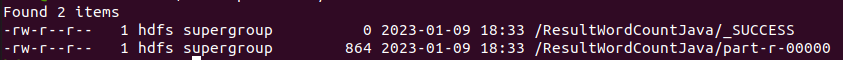
\includegraphics[width=\textwidth]{AryaSaputra/cek hasil resultwordcountjava}
\caption{Hasil Perhitungan dengan WordCount Hadoop}
\label{gam:result wordcount java}
\end{figure}

\vspace*{-1cm}
\begin{figure}[!ht]
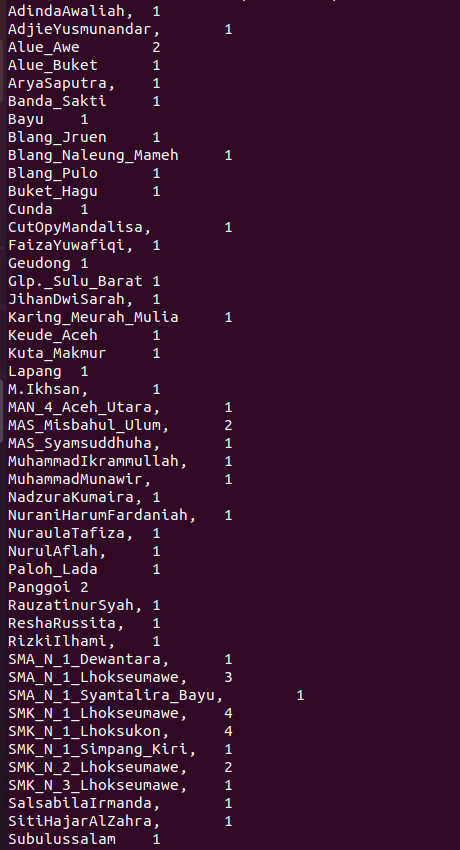
\includegraphics[width=.7\textwidth]{AryaSaputra/hasil wordcount java}
\caption{Hasil Perhitungan dengan WordCount Hadoop}
\label{gam:result wordcount java}
\end{figure}

\vspace*{-.5cm}
\begin{figure}[!ht]
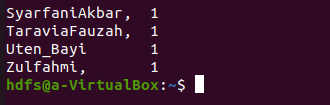
\includegraphics[width=.7\textwidth]{AryaSaputra/hasil wordcount java1}
\caption{Hasil Perhitungan dengan WordCount Hadoop}
\label{gam:result wordcount java}
\end{figure}
\end{enumerate}

\clearpage
\newday{\textbf{22 Desember 2022} - Instalasi Apache Spark (PySpark)}
\begin{enumerate}
\item Kendala dan Solusi \\
Saat melakukan praktikum instalasi apache spark tidak ada kendala saat melakukan pratikum.

\item Kesimpulan \\
Proses penginstalan Apache Spark berhasil dilakukan tanpa adanya kendala satupun

\begin{figure}[!ht]
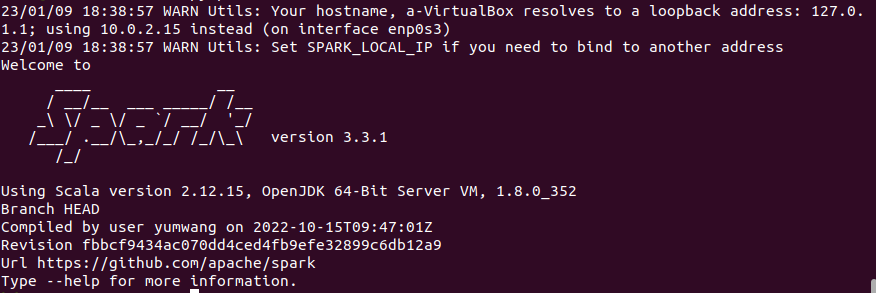
\includegraphics[width=\textwidth]{AryaSaputra/spark}
\caption{Hasil instalasi apache spark}
\label{gam:instalasi apache spark}
\end{figure}
\end{enumerate}


\clearpage
\newday{\textbf{23 Desember 2022}- Program WordCount dengan Python}
\begin{enumerate}
\item Kendala dan Solusi \\
tidak ada kendala saat melakukan pratikum resultwordcountpython.

\item Kesimpulan \\
setelah melakukan percobaan dari tahap awal sampai selesai, kemudian melakukan pengecekan hasil dan melihat hasil word count dengan python. jika hasilnya muncul dan sesuai maka pratikan telah berhasil melakukan percobaan word count dengan python.

\begin{figure}[!ht]
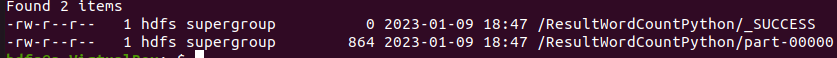
\includegraphics[width=\textwidth]{AryaSaputra/cek hasil resultwordcountpython}
\caption{Hasil wordcountpython}
\label{gam:wordcountpython}
\end{figure}

\vspace*{-1cm}
\begin{figure}[!ht]
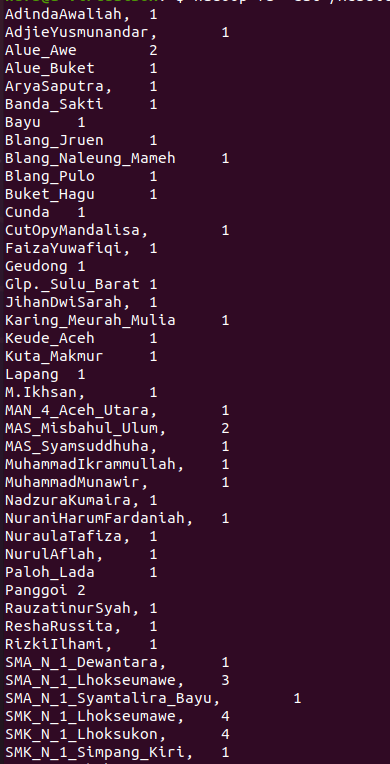
\includegraphics[width=.55\textwidth]{AryaSaputra/hasil result wordcount python}
\caption{Hasil wordcountpython}
\label{gam:wordcountpython}
\end{figure}

\vspace*{-.5cm}
\begin{figure}[!ht]
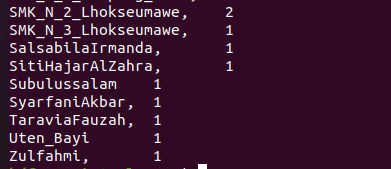
\includegraphics[width=.55\textwidth]{AryaSaputra/hasil result wordcount python1}
\caption{Hasil wordcountpython}
\label{gam:wordcountpython}
\end{figure}
\end{enumerate}

\clearpage
\newday{\textbf{2 Januari 2023} WordCount dengan PySpark}
\begin{enumerate}
\item Kendala dan Solusi \\
tidak ada kendala saat melakukan pratikum.

\item Kesimpulan
\newline Berhasil menjalankan program wordcountpyspark.

\begin{figure}[!ht]
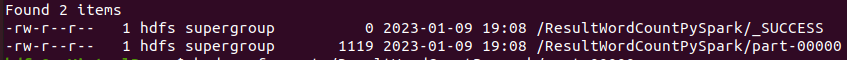
\includegraphics[width=\textwidth]{AryaSaputra/cek hasil rasultwordcountpyspark}
\caption{Hasil resultwordcountpyspark}
\label{gam:resultwordcountpyspark}
\end{figure}

\vspace*{-1cm}
\begin{figure}[!ht]
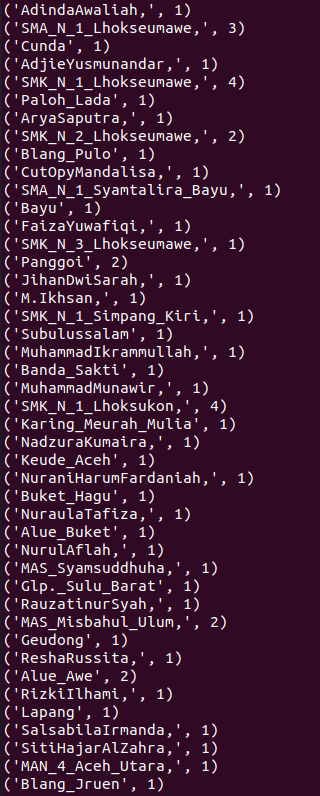
\includegraphics[width=.55\textwidth]{AryaSaputra/hasil resultwordcountpyspark}
\caption{Hasil resultwordcountpyspark}
\label{gam:resultwordcountpyspark}
\end{figure}

\vspace*{-.5cm}
\begin{figure}[!ht]
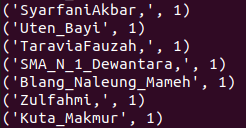
\includegraphics[width=.55\textwidth]{AryaSaputra/hasil resultwordcountpyspark1}
\caption{Hasil resultwordcountpyspark}
\label{gam:resultwordcountpyspark}
\end{figure}
\end{enumerate}
